\documentclass[]{book}
\usepackage{lmodern}
\usepackage{amssymb,amsmath}
\usepackage{ifxetex,ifluatex}
\usepackage{fixltx2e} % provides \textsubscript
\ifnum 0\ifxetex 1\fi\ifluatex 1\fi=0 % if pdftex
  \usepackage[T1]{fontenc}
  \usepackage[utf8]{inputenc}
\else % if luatex or xelatex
  \ifxetex
    \usepackage{mathspec}
  \else
    \usepackage{fontspec}
  \fi
  \defaultfontfeatures{Ligatures=TeX,Scale=MatchLowercase}
\fi
% use upquote if available, for straight quotes in verbatim environments
\IfFileExists{upquote.sty}{\usepackage{upquote}}{}
% use microtype if available
\IfFileExists{microtype.sty}{%
\usepackage{microtype}
\UseMicrotypeSet[protrusion]{basicmath} % disable protrusion for tt fonts
}{}
\usepackage[margin=1in]{geometry}
\usepackage{hyperref}
\hypersetup{unicode=true,
            pdftitle={Seoul Data Catalogue},
            pdfauthor={신혜섭-Hyesop Shin},
            pdfborder={0 0 0},
            breaklinks=true}
\urlstyle{same}  % don't use monospace font for urls
\usepackage{natbib}
\bibliographystyle{apalike}
\usepackage{longtable,booktabs}
\usepackage{graphicx,grffile}
\makeatletter
\def\maxwidth{\ifdim\Gin@nat@width>\linewidth\linewidth\else\Gin@nat@width\fi}
\def\maxheight{\ifdim\Gin@nat@height>\textheight\textheight\else\Gin@nat@height\fi}
\makeatother
% Scale images if necessary, so that they will not overflow the page
% margins by default, and it is still possible to overwrite the defaults
% using explicit options in \includegraphics[width, height, ...]{}
\setkeys{Gin}{width=\maxwidth,height=\maxheight,keepaspectratio}
\IfFileExists{parskip.sty}{%
\usepackage{parskip}
}{% else
\setlength{\parindent}{0pt}
\setlength{\parskip}{6pt plus 2pt minus 1pt}
}
\setlength{\emergencystretch}{3em}  % prevent overfull lines
\providecommand{\tightlist}{%
  \setlength{\itemsep}{0pt}\setlength{\parskip}{0pt}}
\setcounter{secnumdepth}{5}
% Redefines (sub)paragraphs to behave more like sections
\ifx\paragraph\undefined\else
\let\oldparagraph\paragraph
\renewcommand{\paragraph}[1]{\oldparagraph{#1}\mbox{}}
\fi
\ifx\subparagraph\undefined\else
\let\oldsubparagraph\subparagraph
\renewcommand{\subparagraph}[1]{\oldsubparagraph{#1}\mbox{}}
\fi

%%% Use protect on footnotes to avoid problems with footnotes in titles
\let\rmarkdownfootnote\footnote%
\def\footnote{\protect\rmarkdownfootnote}

%%% Change title format to be more compact
\usepackage{titling}

% Create subtitle command for use in maketitle
\newcommand{\subtitle}[1]{
  \posttitle{
    \begin{center}\large#1\end{center}
    }
}

\setlength{\droptitle}{-2em}

  \title{Seoul Data Catalogue}
    \pretitle{\vspace{\droptitle}\centering\huge}
  \posttitle{\par}
    \author{신혜섭-Hyesop Shin}
    \preauthor{\centering\large\emph}
  \postauthor{\par}
      \predate{\centering\large\emph}
  \postdate{\par}
    \date{2018-06-29}

\usepackage{booktabs}

\begin{document}
\maketitle

{
\setcounter{tocdepth}{1}
\tableofcontents
}
\chapter*{Preface}\label{preface}
\addcontentsline{toc}{chapter}{Preface}

Hello, welcome to my website! This site offers a handful of geospatial
data of Seoul, including population, housing, landuse, industry,
traffic, society, hospitality, and environment. Feel free to browse
through this book, and drop me a note if you have any enquiries.

\begin{center}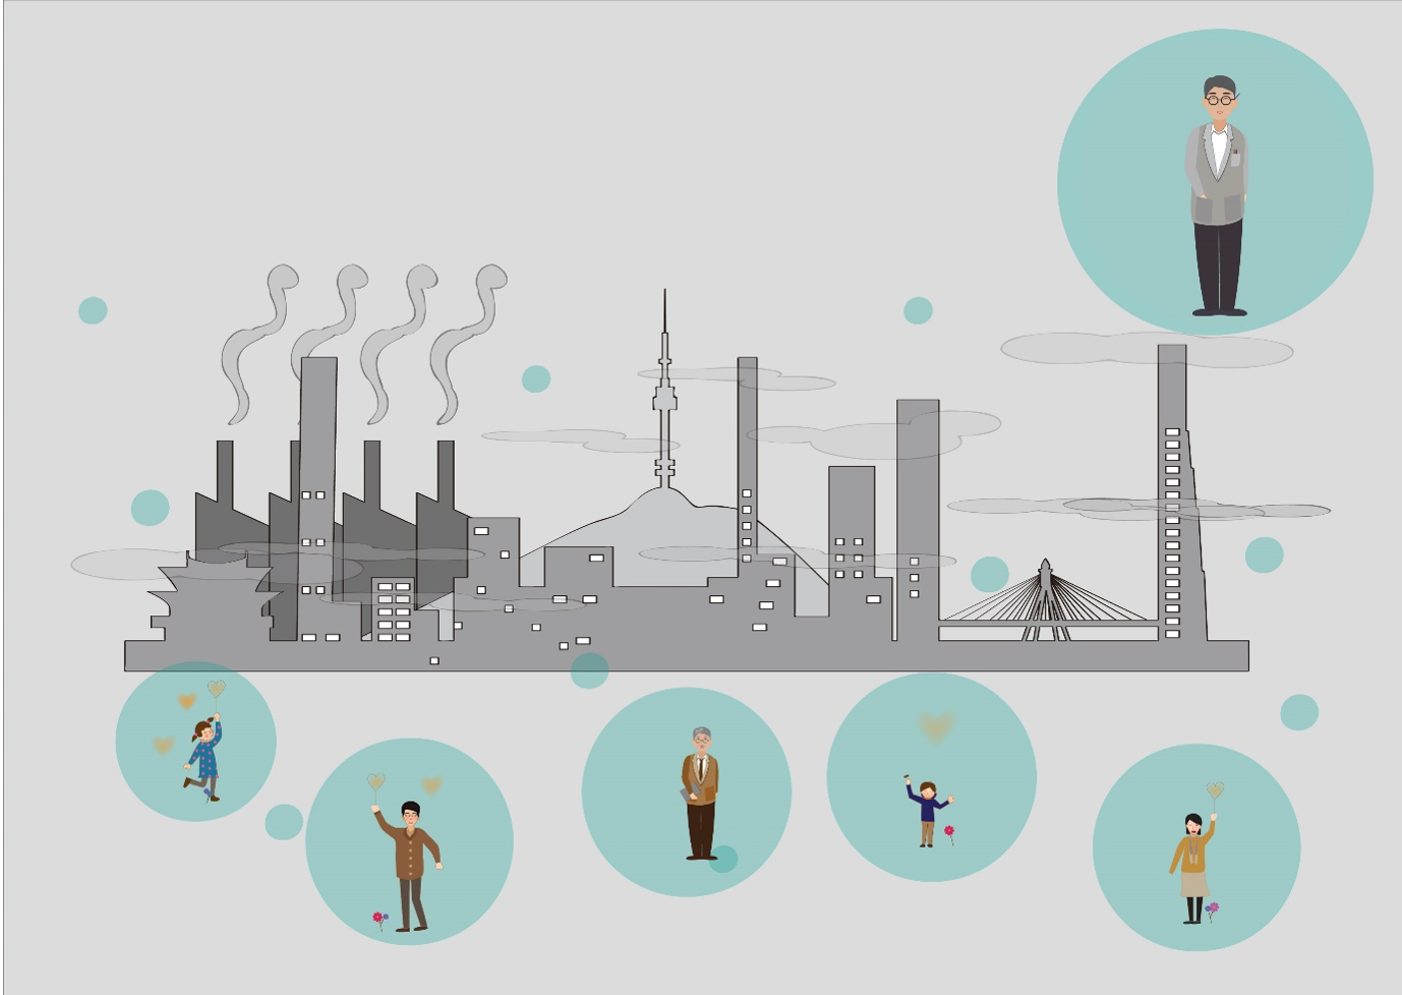
\includegraphics[width=19.47in]{images/01_intro} \end{center}

\chapter{Introduction of Seoul}\label{introduction-of-seoul}

\section{Overview}\label{overview}

\begin{itemize}
\tightlist
\item
  Capital of South Korea
\item
  Area: 605.21 km2 (233.67 sq mi)
\item
  Population: 9,971,111 (678,102 international residents, 2015 NSO)
\item
  Language: Korean
\item
  Currency: Won
\end{itemize}

\section{City Hierarchy}\label{city-hierarchy}

\begin{center}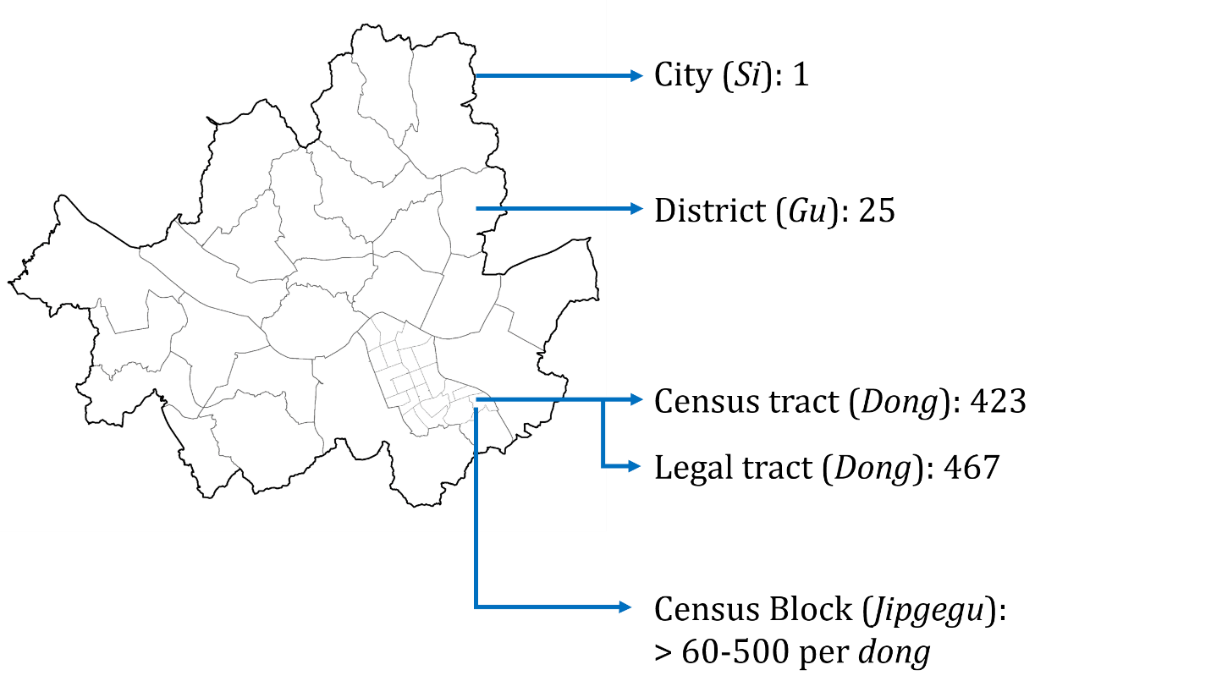
\includegraphics[width=16.82in]{images/02_boundary} \end{center}

The city has four hierarchies, Si, Gu, Dong, and \emph{Jipgegu}, from
city to block level. Within the \emph{Si}(city) scale, Seoul has 25
administrative districts, gu, of which the spatial size is similar to
the boroughs in London. The river Han penetrates horizontally through
the city centre, from east to west, which divides 14 gus to the north,
and 11 to the south.

\chapter{Spatial Boundary}\label{spatial-boundary}

\section{\texorpdfstring{Administrative District
\emph{(Gu)}}{Administrative District (Gu)}}\label{administrative-district-gu}

\emph{Gu}, is a sub-municipal unit in South Korea. \emph{Gu} is normally
regulated when a city has at least a population of 500,000 persons.
Seoul has 25 \emph{gu}s, of which the area and population varies. Seocho
has the largest area (47\(km^2\)) whereas Jung has the smallest
(9.96\(km^2\)). Songpa and Jung are the most and least populated areas,
which are approximately 640,830 and 117,781 persons. To find out more
see \url{https://en.wikipedia.org/wiki/List_of_districts_of_Seoul}.

\begin{figure}

{\centering 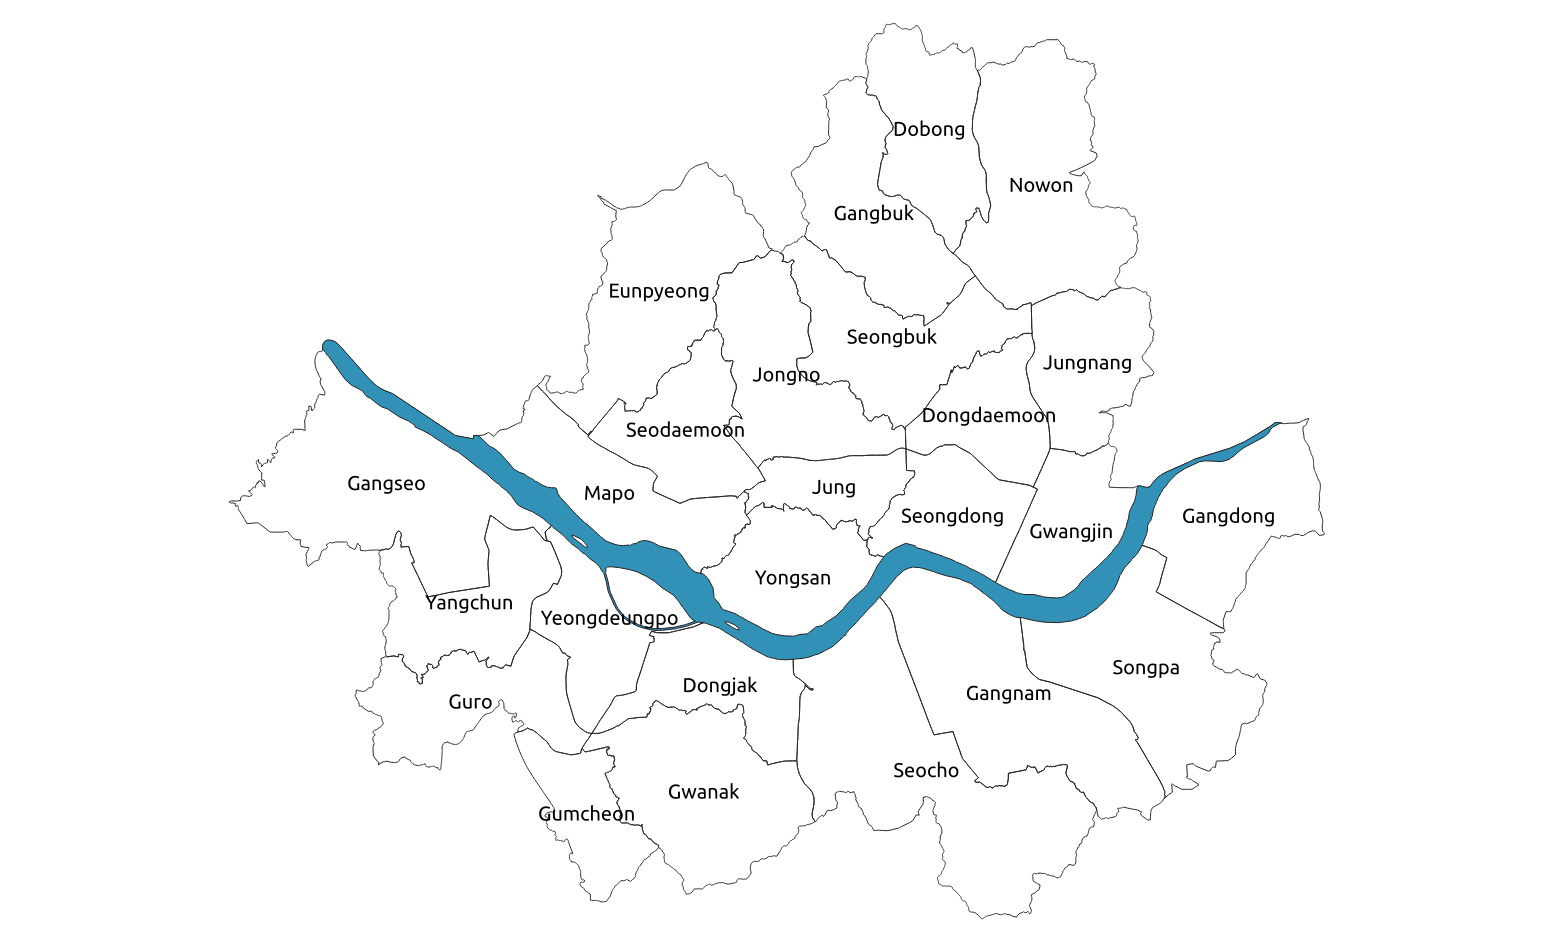
\includegraphics[width=21.57in]{images/03_gu} 

}

\caption{\label{fig:figs} Districts(Gu) in Seoul}\label{fig:unnamed-chunk-3}
\end{figure}

\section{\texorpdfstring{Census tracts
\emph{(Dong)}}{Census tracts (Dong)}}\label{census-tracts-dong}

\emph{Dong}, known as census tracts, are the smallest boundary of which
the authority is owned by the urban government. Each gu comprises two
types of boundaries as \emph{Hengjeong dong}s and \emph{Beopjeong
dong}s. \emph{Hengjeong dong}s, sub-municipal districts, were
established for administrative convenience, such as resident
registration. These \emph{dong}s could be consolidated, divided, or
founded due to population increase or decrease e.g.~Jongno 1-2-3-4ga
dong. \emph{Beopjeong dong}s, legal districts, are towns or villages
that were left for historical significance (Legal dongs were based on
cadastral maps made from the Land investigation project during the
Japanese colonial years). Due to its historial and symbolic meanings,
people tend to remember the names easier than administrative ones. As of
2014, Seoul has 424 administrative dongs and 467 legal dongs. Gildong in
Songpa district was most populated area in 2014 at 49,535 persons,
whereas Sogongdong in Jung district was the least populated at 735
persons.

\begin{figure}

{\centering 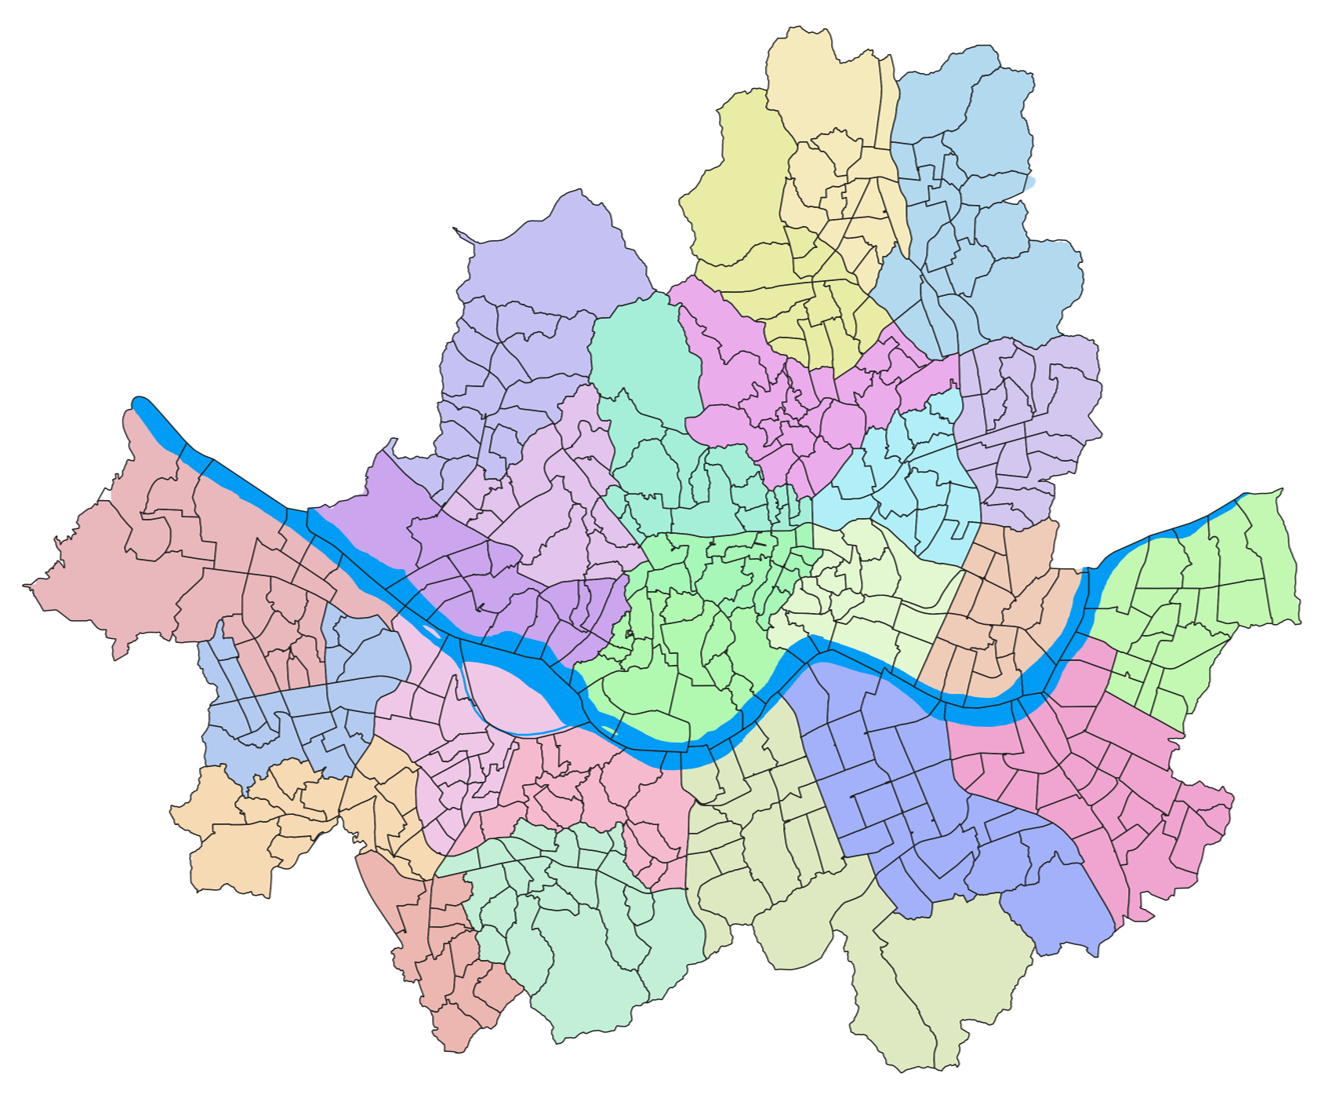
\includegraphics[width=12.99in]{images/04_dong} 

}

\caption{\label{fig:figs} Census tracts(Dong) in Gangnam}\label{fig:unnamed-chunk-4}
\end{figure}

\section{\texorpdfstring{Administrative Census Block
\emph{(Jipgegu)}}{Administrative Census Block (Jipgegu)}}\label{administrative-census-block-jipgegu}

The finest scale is \emph{Jipgegu}, or census block. This boundary is
mainly to retrieve the population from a minimum statistical area, thus
does not function as an administrative unit. Each Jipgegu consists of
60-500 residents, and the boundaries are renewed every year. As of 2013,
Seoul has 16,470 jipgegus. All boundary data were provided in a
shapefile in a 5-year period from 1975-2015, except the \emph{Jipgegu}
where the last update was in 2016.

\begin{figure}

{\centering 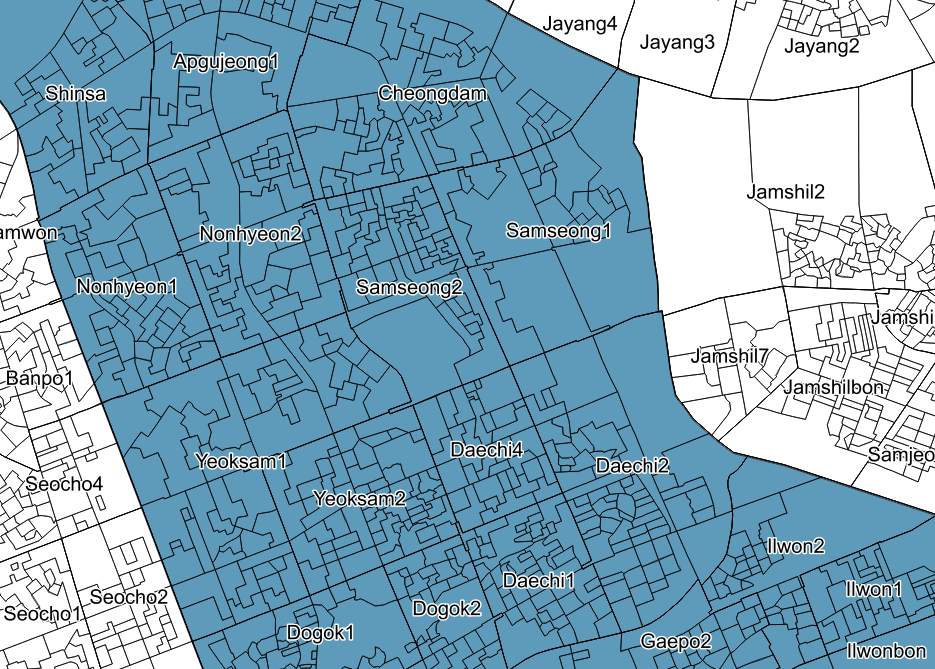
\includegraphics[width=12.99in]{images/05_jip} 

}

\caption{\label{fig:figs} Census block(Jipgyegu) in Gangnam}\label{fig:unnamed-chunk-5}
\end{figure}

\chapter{Population}\label{population}

\section{Population Census}\label{population-census}

Population data of residence

\begin{itemize}
\tightlist
\item
  Reference: Korean Statistics Office
\item
  Time Period : 2011 - 2015
\item
  Data Collected: Monthly
\item
  Data Type : .csv
\item
  Spatial range : Seoul 
\end{itemize}

\begin{longtable}[]{@{}ll@{}}
\toprule
Field & Description\tabularnewline
\midrule
\endhead
std\_yy & Baseline year\tabularnewline
std\_mt & Baseline month\tabularnewline
sexdstn\_cd & Sex\tabularnewline
agrde\_cd & Age group\tabularnewline
rspop\_cnt & Population\tabularnewline
adstrd\_cd & Census tract code\tabularnewline
signgu\_cd & City code\tabularnewline
\bottomrule
\end{longtable}

\section{Employees at Working place}\label{employees-at-working-place}

Data on the number of employees per census block, based on the basic
survey data of the business

• Reference: Seoul city • Time Period : 2011 - 2013 • Data Collected:
Annually • Data Type : .csv • Spatial range : Seoul

\section{De Facto Population}\label{de-facto-population}

구분: 인구/가구 데이터셋명: 생활인구 자료유형: 속성(csv) 시간범위:
2017.01.01-2018.04.18 공간범위: 서울전역 적재주기: 월 제공기관: KT

파일명: - 내국인: SE\_SPOP\_LOCAL\_RESD\_YYMM - 외국단기:
SE\_SPOP\_TEMP\_RESD\_YYMM - 외국장기: SE\_SPOP\_LONG\_RESD\_YYMM -
대도시권 생활인구: SE\_SPOP\_ORGN\_CT\_YYMM - 데이터셋설명: 생활인구란
거주인구가 아닌 실제로 생활하는 인구로, 1시간 단위로 서울시 전체,
자치구별, 행정동별, 집계구별로 서울을 커버하는 KT의 통신기지국(LTE
시그널 데이터 기반)에 존재하는 인구를 기초로 추정함. LTE가입률이
떨어지는 저연령과 고연령층은 주민등록인구비율을 반영하여 생활인구를
대체함. 그리고 장단기체류 외국인은 국내 휴대폰에 가입한 외국인의
이용정보와 국내의 로밍서비스를 받는 외국인 정보를 활용하여 생활인구
추계과정과 동일하게 접근하고 국적별로 보정함. `대도시권' 데이터는
생활인구 데이터에 대도시권의 거주지 코드를 포함한 데이터임 추정된
데이터로 소수점(5자리) 이하값이 있으며, 각 값의 합은 전체합계와 일치하지
않을 수 있음

\chapter{Traffic}\label{traffic}

Traffic GIS DB - O-D Matrix - Traffic Volume (67 within Seoul) - Road
network - Bus(Regular, Intercity)

\section{Traffic facilities}\label{traffic-facilities}

Traffic facilities are the geographic locations of bus stops and subway
stations in Seoul. This dataset is provided by Seoul TOPIS(Transport
Operation and Information Services, 서울시교통정보센터), and KAIS(Korean
Address Information System, 국가주소정보시스템), during the period of
January 2015 - August 2016. The data are saved in an excel sheet and a
shape format.

\begin{itemize}
\tightlist
\item
  EPSG(Coordinates): 5181(Korea 2000 Central Belt)
\end{itemize}

In the folder, you will probably notice two sets of files, which either
starts with TB\_O\_SB\_STATN or TB\_E\_BUSSTOP:

\begin{longtable}[]{@{}lll@{}}
\toprule
Type & Description & Code\tabularnewline
\midrule
\endhead
\texttt{Facilities} & Subway location &
\texttt{TB\_O\_SB\_STATN}\tabularnewline
\texttt{Facilities} & Bus location &
\texttt{TB\_E\_BUSSTOP}\tabularnewline
\bottomrule
\end{longtable}

 * Bus stop: Attributes

\begin{longtable}[]{@{}lll@{}}
\toprule
NO & Attribute Name & Note\tabularnewline
\midrule
\endhead
1 & \texttt{ID} &\tabularnewline
2 & \texttt{Bus\ stop\ number} &\tabularnewline
3 & \texttt{Bust\ stop\ name} &\tabularnewline
4 & \texttt{Year} & Jan.2015-Aug.2016\tabularnewline
5 & \texttt{TM-X} &\tabularnewline
6 & \texttt{TM-Y} &\tabularnewline
\bottomrule
\end{longtable}

\begin{itemize}
\tightlist
\item
  Bus stop: Shape file attributes (EPSG:5181)
\end{itemize}

\begin{longtable}[]{@{}lll@{}}
\toprule
NO & Column Code & Column Name\tabularnewline
\midrule
\endhead
1 & \texttt{YYYYMM} & Year+Month\tabularnewline
2 & \texttt{LINE\_NO} & Bus number\tabularnewline
3 & \texttt{SEQ\_NO} & Order\tabularnewline
4 & \texttt{BUS\_STA\_NM} & Bus stop name\tabularnewline
5 & \texttt{X\_COORD} & X coordinate\tabularnewline
6 & \texttt{Y\_COORD} & Y coordinate\tabularnewline
7 & \texttt{ARSID} & Reference\tabularnewline
\bottomrule
\end{longtable}

\begin{itemize}
\tightlist
\item
  Subway: Attributes
\end{itemize}

\begin{longtable}[]{@{}lll@{}}
\toprule
NO & Attribute Name & Note\tabularnewline
\midrule
\endhead
1 & \texttt{ID} &\tabularnewline
2 & \texttt{Station\ name} &\tabularnewline
3 & \texttt{Line\ number} &\tabularnewline
4 & \texttt{Year} & Jan.2015-Aug.2016\tabularnewline
5 & \texttt{TM-X} &\tabularnewline
6 & \texttt{TM-Y} &\tabularnewline
\bottomrule
\end{longtable}

\begin{itemize}
\tightlist
\item
  Subway: Shape file attributes (EPSG:5181)
\end{itemize}

\begin{longtable}[]{@{}lll@{}}
\toprule
NO & Column Code & Column Name\tabularnewline
\midrule
\endhead
1 & \texttt{GU\_NM} & Year+Month\tabularnewline
2 & \texttt{GU\_CD} & Bus number\tabularnewline
3 & \texttt{SUB\_STA\_SN} & Order\tabularnewline
4 & \texttt{KOR\_SUB\_NM} & Bus stop name\tabularnewline
5 & \texttt{Point\_X} & X coordinate\tabularnewline
6 & \texttt{Point\_Y} & Y coordinate\tabularnewline
\bottomrule
\end{longtable}

\chapter{Pollution}\label{pollution}

\chapter{Patients}\label{patients}

HIRA data

\bibliography{book.bib,packages.bib}


\end{document}
